\selectlanguage{ngerman}%
\frenchspacing%
\begin{ledgroupsized}[r]{120mm}%
\footnotesize%
\pstart%
\noindent\textbf{Überlieferung:}%
\pend%
\end{ledgroupsized}%
\begin{ledgroupsized}[r]{114mm}%
\footnotesize%
\pstart%
\parindent -6mm%
\makebox[6mm][l]{\textit{L}}%
Aufzeichnung:
LBr~413 Bl.\;48.
Ein Blatt 2\textsuperscript{o};
Wassezeichen. %
Eine Seite auf Bl.\;\href{\Scan{LBr_413_048v}}{48\,v\textsuperscript{o}}.
Bl.\;\href{\Scan{LBr_413_048r}}{48\,r\textsuperscript{o}} überliefert eine Aufzeichnung medizinischen Inhalts,
die voraussichtlich in einem späteren Band von \textit{LSB}\;VIII erscheinen wird.
\pend%
\end{ledgroupsized}%
\selectlanguage{latin}%
\frenchspacing%
\vspace{8mm}%
\normalsize%
\pstart%
\noindent%
\edtext{%
\lbrack%
\href{\Scan{LBr_413_048v}}%
{48\,v\textsuperscript{o}}%
\rbrack
Mirum et expectationi%
\indexS{expectatio}
contrarium habetur%
}{%
\lemma{\lbrack\href{\Scan{LBr_413_048v}}{48\,v\textsuperscript{o}}\rbrack}%
\Bfootnote{%
\textit{(1)}~Cum mirum %
\textit{(2)}~Mirum et expectationi contrarium %
\textit{(a)}~videatur %
\textit{(b)}~sit %
\textit{(c)}~habetur%
~\textit{L}%
}}
Hydrargyrum in Barometro ascendere%
\indexS{hydrargyrym ascendens}\indexS{hydrargyrym in barometro}%
\indexS{barometrum}
sereno coelo,%
\indexS{coelum serenum}
descendere%
\indexS{hydrargyrym descendens}\indexS{hydrargyrym in barometro}
pluvio,%
\indexS{coelum pluvium}
aut pluviam minante:%
\indexS{coelum minans pluviam}%
\indexS{pluvia}
Cum aer pluvius%
\indexS{aer pluvius}
magis oneratus aquosis vaporibus,%
\indexS{aer oneratus vaporibus}%
\indexS{vapor aquosus}
\edtext{%
et graviore%
}{%
\lemma{et}\Bfootnote{%
\textit{(1)}~majore %
\textit{(2)}~graviore%
~\textit{L}%
}}
adeo columna%
\indexS{columna aeris}%
\lbrack,\rbrack\
oppositum sibi velut in lance%
\indexS{lanx}
\edtext{%
Mercurium%
\indexS{mercurius impulsus pressione aeris}%
}{%
\lemma{Mercurium}%
\Bfootnote{\textit{erg.\;L}%
}}
pressione sua%
\indexS{pressio aeris}
sursum impulsurus%
\indexS{aer impellens mercurium sursum}
videatur.
\edlabel{LBr_413_048_048v_Schelh-1}%
\edtext{%
Variae viris eruditissimis%
\indexS{vir eruditus}
natae sunt sententiae%
\indexS{sententia}
et contentiones,%
\indexS{contentio}
phaenomeni explicandi causa,%
\indexS{causa phaenomeni explicandi}%
\indexS{phaenomenon explicandum}%
}{%
\lemma{Variae \lbrack...\rbrack\ causa}%
\Cfootnote{%
Siehe oben, die Aufzeichnung N.\;\ref{60267}, \refpassage{LH_37_04_149-150_149r_ersterTeil-1}{LH_37_04_149-150_149r_ersterTeil-2} (samt Erläuterungen).
Dort legt Leibniz in Anlehnung an
\textsc{B.\;Ramazzini}, \textit{Ephemerides barometricae}
(Modena 1695;\cite{01516} Augsburg 1696)\cite{01517}
die Debatte über das kontraintuitiven Verhalten des Luftgewichts ausführlich dar.%
}}
de quibus scripta%
\indexS{scripta mutua}
\edtext{%
nupera et mutua%
}{%
\lemma{nupera et mutua}%
\Bfootnote{%
\textit{erg.\;L}%
}}
virorum clarissimorum%
\indexS{vir clarus}
\edtext{%
Camerarii,%
\indexN{\textls{Camerarius}, Rudolf Jakob 1665\textendash1721}%
}{%
\lemma{Camerarii}%
\Cfootnote{%
Siehe
\textsc{R.\:J.\;Camerarius}, \textit{Ephemerides meteorologicae} (Augsburg 1696).\cite{01445}%
}}
\edtext{%
Ramazzini,%
\indexN{\textls{Ramazzini} (Ramazzinus), Bernardino 1633\textendash1714}
\edtext{%
Schelhameri%
\indexN{\textls{Schelhammer} (Schelhammerus), Günther Christoph 1649\textendash1716}
legi%
}{%
\lemma{Schelhameri}%
\Bfootnote{%
\bars{et Camerarii~\textit{gestr.}} legi%
\textit{L}%
}}%
}{%
\lemma{Ramazzini, Schelhameri}%
\Cfootnote{%
Zwischen B.\;Ramazzini und G.\:C.\;Schelhammer entwickelte sich ab 1697 eine gelehrte Auseinandersetzung über die Ursachen des "barometrischen Paradoxons".
Siehe über die daraus entstandene Schriften oben, die editorische Einleitung zu N.\;\ref{paradoxon_intro}, \refpassage{paradoxon_RamaSchel-fhg-1}{paradoxon_RamaSchel-fhg-3}.%
}}
possunt.%
\edlabel{LBr_413_048v_01a}%
\edlabel{LBr_413_048_048v_Schelh-2}%
\edtext{}{%
\xxref{LBr_413_048v_01a}{LBr_413_048v_01b}%
\lemma{possunt.}%
\Bfootnote{%
\lbrack/\rbrack\
\textit{(1)}~Ego %
\textit{(2)}~Mihi visum est%
~\textit{L}}}%
\pend%
\pstart%
Mihi visum est%
\edlabel{LBr_413_048v_01b}
rem Mechanico quodam Experimento posse illustrari.%
\indexS{experimentum mechanicum}
\edtext{%
In bilance \textit{B},%
\indexS{bilanx}%
}{%
\lemma{In bilance \textit{B}}%
\Cfootnote{%
Vgl. das Diagramm \lbrack\textit{Fig.\:1}\rbrack.%
}}
sit ab una parte pondus \textit{P},%
\indexS{pondus aequilibratum in bilance}
ab altera,
in aequilibrium suspensus,%
\indexS{aequilibrium in bilance}
tubus%
\indexS{tubus suspensus in aequilibrium}
\edtext{%
vitreus%
\indexS{tubus vitreus}%
}{%
\lemma{vitreus}%
\Bfootnote{%
\textit{erg.\;L}%
}}
\textit{T}
satis longus,
aqua repletus,%
\indexS{tubus repletus aqua}
in quo natet vasculum \textit{V}%
\indexS{vasculum natans}
cavum atque pertusum foramine%
\indexS{vasculum pertusum foramine}
ita
\edtext{%
obturato,%
\indexS{foramen vasculi obturatum}
veluti charta%
\indexS{charta obturans foramen}
aut alio obstaculo%
\indexS{obstaculum obturans foramen}%
\indexS{obstaculum per quod aqua transit} %
per quod %
filtratione%
\indexS{filtratio}
aut solutione%
\indexS{solutio} %
mox transire possit aqua,%
\indexS{aqua transiens per obstaculum}%
\indexS{aqua transiens filtratione aut solutione}
ut scilicet
aliquamdiu exclusa,
mox illabatur.%
\indexS{aqua illabans in vasculum}
Res ita temperabitur%
\indexS{res temperata}%
}{%
\lemma{obturato,}%
\Bfootnote{%
\textit{(1)}~ut %
\textit{(a)}~paulatim illabi possit aqua %
\textit{(b)}~aqua aliquamdiu exclusa mox illabatur %
\textit{(2)}~\bars{veluti charta aut alio \textit{erg.}} obstaculo, per %
\lbrack...\rbrack\ aut solutione %
\bars{mox \textit{erg.}} transire possit %
\lbrack...\rbrack\ mox illabatur %
\textit{(a)}~; ac demu %
\textit{(b)}~. Res ita temperabitur%
~\textit{L}%
}}
ut%
\lbrack,\rbrack\
\edtext{%
dum vasculum adhuc in summo natat,%
\indexS{vasculum natans}
sint \textit{T} et \textit{P} in aequilibrio.%
\indexS{aequilibrium in bilance}%
}{%
\lemma{dum}%
\Bfootnote{%
\textit{(1)}~aqua %
\textit{(2)}~vasculum 
\textit{(a)}~natat %
\textit{(b)}~sit %
\textit{(c)}~\textit{P} et \textit{T} sint in aequ %
\textit{(3)}~adhuc in %
\lbrack...\rbrack\ in aequilibrio.%
~\textit{L}%
}}
\pend%
\newpage%
\pstart%
\edtext{Dico%
\lbrack:\rbrack\
ubi aqua irrepserit%
\indexS{aqua irrepens in vasculum}
secuto ac durante descensu vasculi,%
\indexS{descensus vasculi in aqua}%
\indexS{vasculum descendens in aqua}
descensurum esse pondus~\textit{P},
atque adeo ipso praevalente%
\indexS{pondus praevalens in bilance} %
aequilibrium esse cessaturum,%
\indexS{aequilibrium cessans}%
}{%
\lemma{Dico}%
\Bfootnote{%
\textit{(1)}~cessante %
\textit{(2)}~durante descensu %
\textit{(3)}~ubi aqua irrepserit %
\bars{secuto ac\textit{~erg.}} durante descensu %
\textit{(a)}~vasculi aequilibrium esse cessaturum, %
\textit{(aa)}~et pondus~\textit{P} praevaliturum %
\textit{(bb)}~praevalituro pondere~\textit{P} %
\textit{(b)}~vasculi, descensurum %
\lbrack...\rbrack\ esse cessaturum,%
~\textit{L}%
}}
nec rediturum%
\indexS{reditus aequilibrii}
donec vasculum attigerit fundum tubi.%
\indexS{fundus tubi}%
\edtext{}{%
\lemma{\textit{Am Rand, abbrechend und gestrichen:}}%
\Afootnote{%
\footnotesize{%
Sunt \textlangle tamen\textrangle\ et alii modi quibus}%
}}
Cuius rei ratio est,%
\indexS{ratio rei}
quod
durante descensu%
\indexS{descensus vasculi in aqua}
vasculum%
\indexS{vasculum sustentum in aequilibrium}
\edtext{%
a pondere \textit{P}%
}{%
\lemma{a pondere \textit{P}}%
\Bfootnote{%
\textit{erg.\;L}%
}}
non sustinetur,
itaque
quantum gravitatis in vasculo est%
\indexS{gravitas vasculi descendentis}
dum descendit,
tantum ponderis parti \textit{T} in balance%
\indexS{balanx}
detractum iri.%
\indexS{pondus detractum}%
\indexS{detractio ponderis}%
\pend%
\begin{edfigure}[2.0em][1.5em]
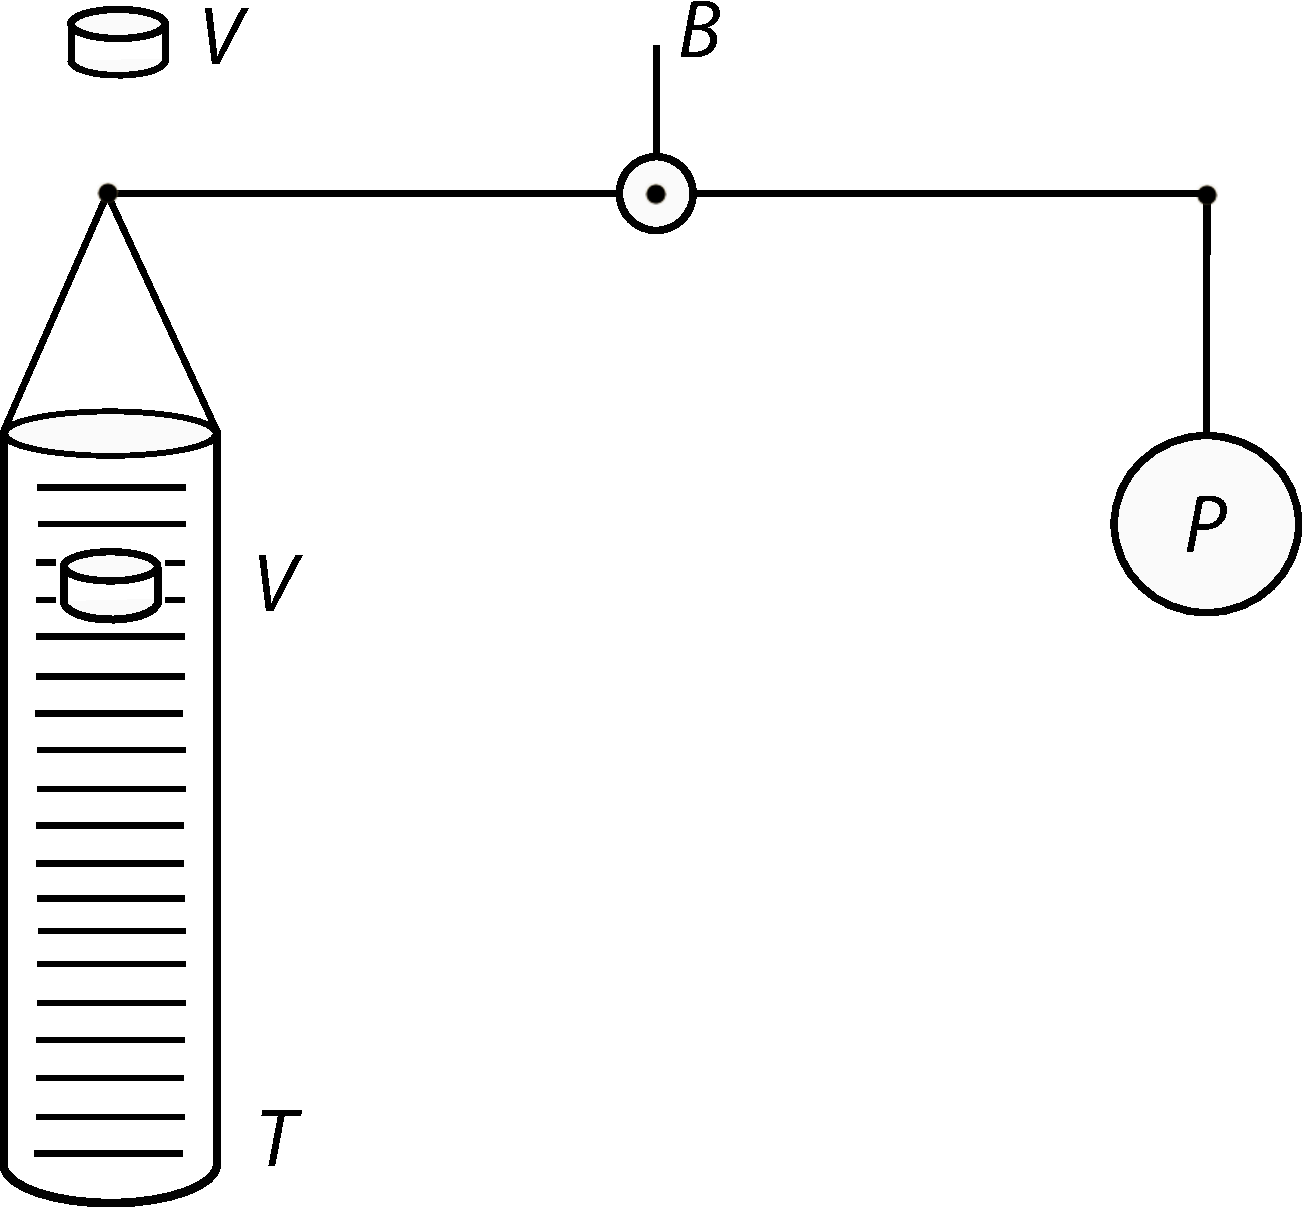
\includegraphics[width=0.42\textwidth]{gesamttex/edit_VIII-4/images/LBr_413_048_d_048v.pdf}
\edcaption[-0.5em]{\lbrack \textit{Fig.\:1}\rbrack}%
\end{edfigure}%
\pstart%
Haec in rem nostram transferamus.%
\indexS{res nostra}
\edtext{%
Ponderi \textit{P}%
\indexS{pondus aequilibratum in bilance}
respondet Mercurius in Barometro;%
\indexS{mercurius in barometro}%
\indexS{barometrum}
columnae in tubo \textit{T}%
\indexS{columna in tubo}
respondet aeris columna,%
\indexS{columna aeris}%
}{%
\lemma{Ponderi \textit{P}}%
\Bfootnote{%
\textit{(1)}~in Barometri phaenomeno proposito %
\textit{(2)}~respondet %
\textit{(a)}~Mer %
\textit{(b)}~Hydrargyrus %
\textit{(c)}~Mercurius in %
\textit{(aa)}~Tu %
\textit{(bb)}~Barometro; %
\textit{(aaa)}~tubo \textit{T} respondet aeris %
\textit{(bbb)}~columnae in %
\lbrack...\rbrack\ aeris columna,%
~\textit{L}%
}}
vasculo%
\indexS{vasculum natans}
respondent aqueae guttae per aerem dispersae.%
\indexS{gutta aquea}%
\indexS{guttae dispersae per aerem}%
\indexS{dispersio guttarum per aerem}
\edtext{%
Haec dum in minutissimas partes sunt divisae%
\indexS{gutta divisa in partes minutas}%
}{%
\lemma{Haec}%
\Bfootnote{%
\textit{(1)}~dum exiguae adhu %
\textit{(2)}~dum in %
\lbrack...\rbrack\ sunt divisae%
~\textit{L}%
}}
vim descendendi non habent,%
\indexS{vis descendendi guttarum in aere}%
\indexS{gutta carens vi descendendi}
quia plus habent superficiei
quam pro mole,%
\indexS{proportio superficiei ad molem}
atque adeo aeris cohaesionem%
\indexS{cohaesio aeris} %
et%
\lbrack,\rbrack\
quae in omni fluido est,%
\indexS{cohaesio fluidi}
velut glutinositatem quantumvis exiguam%
\indexS{glutinositas fluidi exigua}
vincere non possunt,
natantque;%
\indexS{gutta natans in aere}
ne dicam huc illuc volitare%
\indexS{gutta volitans in aere} %
ut pulveris atomos %
\indexS{atomus pulveris}%
\indexS{pulvis}
quas videmus in sole,%
\indexS{sol}
\edtext{%
nonnullas etiam esse rarefactas.%
\indexS{gutta rarefacta}%
}{%
\lemma{nonnullas etiam esse rarefactas}%
\Bfootnote{%
\textit{erg.\;L}%
}}
Sed ubi multae particulae exiguae aquosi vaporis%
\indexS{particulae vaporis collectae}%
\indexS{vapor aquosus}
\edtext{%
condensati%
\indexS{vapor condensatus}%
}{%
\lemma{condensati}%
\Bfootnote{%
\textit{erg.\;L}%
}}
collectae sunt
\edtext{%
in unius guttulae%
}{%
\lemma{in}%
\Bfootnote{%
\textit{(1)}~unam %
\textit{(2)}~unius guttulae%
~\textit{L}%
}}
rudimentum,%
\indexS{rudimentum guttulae}
jam descendunt%
\indexS{particulae vaporis descendentes}
atque inter descendendum
etiam augentur%
\lbrack,\rbrack\
ut procurrens pila nivis.%
\indexS{pila nivis}%
\indexS{nix}
Durante autem hoc innumerabilium guttarum descensu%
\indexS{descensus guttarum innumerabilium}
tantum levior fit
\edtext{%
columna,%
\indexS{columna aeris}
quantum%
}{%
\lemma{columna}%
\Bfootnote{%
\bars{fit \textit{streicht Hrsg.}}, quantum%
~\textit{L}%
}}
est ponderis in descensu guttarum,%
\indexS{pondus guttarum descendentium}%
\indexS{descensus guttarum innumerabilium}
quae scilicet amplius a columna%
\indexS{columna aeris}
non sustinentur.
Atque hinc vaticinatur Barometrum futuram pluviam,%
\indexS{barometrum vaticinans pluviam}%
\indexS{pluvia futura}
quod jam sentit hanc columnae aereae%
\indexS{columna aerea}
ut sic dicam alleviationem,%
\indexS{alleviatio columnae aereae}
\edtext{%
antequam cadendo ad nos%
}{%
\lemma{antequam}%
\Bfootnote{%
\textit{(1)}~ad nos %
\textit{(2)}~cadendo %
\textit{(a)}~crescendoque %
\textit{(b)}~ad nos%
~\textit{L}%
}}
perveniant guttulae %
\indexS{guttula cadens}
et %
quantum ad pluviam%
\indexS{pluvia futura}
\edtext{%
aut nivem%
\indexS{nix}%
}{%
\lemma{aut nivem}%
\Bfootnote{%
\textit{erg.\;L}%
}}
satis est %
cadendo
\edlabel{LBr_413_048_048v_sviu-1}%
\edtext{}{%
\xxref{LBr_413_048_048v_sviu-1}{LBr_413_048_048v_sviu-2}%
\lemma{crescant.}%
\Bfootnote{%
\textit{(1)}~Hinc et ventus ingens columnam\indexS{ventus ingens} %
\textit{(2)}~Sed ubi serenitas vapores %
\bars{aquosos \textit{erg.}} rursus comminuit %
\lbrack...\rbrack\ aeris reddant leviorem,%
~\textit{L}%
}}%
crescant.
Sed ubi serenitas%
\indexS{serenitas}
vapores aquosos%
\indexS{vapor aquosus}
rursus comminuit%
\indexS{vapor comminutus}
atque dispersit,%
\indexS{vapor dispersus}
sive aestate%
\indexS{aestas}
sive hyeme,%
\indexS{hyems}
manifestum est
rursus sustineri eos columna,%
\indexS{vapor sustentus columna aerea}
et gravitatem ei redire.%
\indexS{gravitas redita}%
\pend%
\pstart%
Patet hinc etiam
cur venti columnam aeris reddant leviorem,%
\indexS{ventus reddens columnam aeris leviorem}%
\indexS{columna aeris reddita levior ventis}%
\edlabel{LBr_413_048_048v_sviu-2}
nempe
quantum ipsi sustinent,
\edtext{%
tantum resistentiae ex columna aeris%
\indexS{resistentia columnae aeris}
Mercurius in Barometro%
\indexS{mercurius in barometro}%
\indexS{barometrum}
sibi detractum sentit,%
}{%
\lemma{tantum}%
\Bfootnote{%
\textit{(1)}~non sentit resti %
\textit{(2)}~resistentiae ex %
\lbrack...\rbrack\ detractum sentit,%
~\textit{L}}}
descensuque testatur.%
\indexS{descensus mercurii}
Et perinde est
ac si extranea vis%
\indexS{vis extranea}%
\indexS{vis sustinens aquam in tubo}
aquam in Tubo \textit{T}%
\indexS{aqua sustenta in tubo}
pro bona parte sustineret,
haustro fortassis aliquo immerso %
\indexS{haustrum immersum}
\edtext{%
quo aqua sursum traheretur.%
\indexS{aqua tracta sursum}%
}{%
\lemma{quo}%
\Bfootnote{%
\textit{(1)}~extrahere %
\textit{(2)}~illa %
\textit{(3)}~aqua sursum traheretur.%
~\textit{L}%
}}
Tantum enim vinceret pondus oppositum \textit{P}%
\indexS{pondus vincens in bilance}
descenderetque. 
\edtext{%
Hinc maxima futura est
\textls{Barometri%
\indexS{utilitas barometri ad praevidendas tempestates}%
\indexS{barometrum}
utilitas}%
}{%
\lemma{Hinc}%
\Bfootnote{%
\textit{(1)}~summa utilitas %
\textit{(2)}~\bars{Hinc \textit{streicht Hrsg.}} maxima %
\textit{(a)}~erit %
\textit{(b)}~es %
\textit{(c)}~futura est \textls{Barometri utilitas}%
~\textit{L}%
}}
\textls{in mari%
\indexS{mare}
ad praevidendas%
\indexS{tempestas praevidenda}
tempestates,}
jam aliquot horae sufficere possunt,
si non ut portus petatur%
\indexS{portus petitus}%
\lbrack,\rbrack\
saltem %
ut recedatur a scopulis%
\indexS{scopulus}
syrtibusque%
\indexS{syrtis}
\edtext{%
et navis paretur ad sustinendam%
\indexS{navis parata ad vim procellae sustinendam}%
}{%
\lemma{et}%
\Bfootnote{%
\textit{(1)}~ad sustinenda %
\textit{(2)}~navis paretur ad sustinendam%
~\textit{L}%
}}
vim procellae.%
\indexS{vis procellae}%
\indexS{procella}
Ut mirum sit
per tot jam annos
rem tantae utilitatis esse neglectam.%
\indexS{res neglecta}%
\pend%
\selectlanguage{latin}%
\frenchspacing%
\normalsize%
